% \textcolor{red}{This needs some rework - maybe we can make some kind of table with what algorithm each planning uses?}\\
% \textcolor{red}{TODO: mention here that the code is split into multiple packages which are kinda standalone projects by themselves. Maybe list them here too.}
% \begin{itemize}
%     \item[-] Application Interface component
%     \item[-] ``Nurse rostering'' problem solving component
%     \item[-] ``Traveling salesman'' problem solving component
%     \item[-]``Task assigning'' problem solving component
%     \item[-]``Cloud balancing'' problem solving component
%     \item[-]``Conference scheduling'' problem solving component
%     \item[-]``Vehicle routing'' problem solving component
%     \item[-]``Hospital bed planning'' problem solving component
%     \item[-]``Machine reassignment'' problem solving component
%     \item[-]``Course timetabling'' problem solving component
%     \item[-]``Rock tour'' problem solving component
%     \item[-]``Project job scheduling'' problem solving component
%     \item[-]``N queen'' problem solving component
%     \item[-]``Exam timetabling'' problem solving component
%     \item[-]``Coach shuttle gathering'' problem solving component
%     \item[-]``Cheap time scheduling'' problem solving component
%     \item[-]``Scrabble compacter'' problem solving component
%     \item[-]``Meeting scheduling'' problem solving component
%     \item[-]``Traveling tournamentt'' problem solving component
%     \item[-]``Investment allocation'' problem solving component
%     \item[-]``Dinner party'' problem solving component
%     \item[-]``Tennis club schedulign'' problem solving component
%     \item[-] ``Flight crew scheduling'' problem solving component
% \end{itemize}
We present an initial overview of the architectural components of the system, based on the documentation as well as experience with running the application.

\subsection{Example applications from OptaPlanner: Running one instance}
In order to get a better understanding of the system, we briefly present a simple example of how OptaPlanner can be used to solve an NP-problem. Namely, we want to assign taks to different employees based on their set of skills and availabilities.
Therefore we have selected ``\textit{Task assigning}'' from the possible options in Figure \ref{fig:OP_UI}. \\\\
When we first upload the file, the system sees a number of employees, a set of tasks that need to be completed and a few different timeslots (Figure \ref{fig:task1}). When we click on {\small\MakeUppercase{Solve}}, we see OptaPlanner solving the task assignment for us (Figure \ref{fig:task2}). The coloured rectangles represent a specific skill. Note how the set of skills that are required for a task matches the set of skills of the employee that is assigned the task. This proves that OptaPlanner makes sure that the necessary constraints are met.
\noindent The application can provide a solution for new incoming tasks as well, and even extend the timeslots once they are filled up for every employee. Note that this is only one of the multiple problems that the system can tackle. Other problem types have different representations and different layouts. Nonetheless, the task of the end-user remains the same: upload the problem file and see how OptaPlanner provides a solution for it. \\
One of the key advantages of OptaPlanner is how the system is \textit{standalone}, on the one hand, as it can be installed and used on its own, but it is also \textit{embeddable}, so that developers can access different internal components and algorithm from the system.
\begin{figure}[H]
    \centering  
    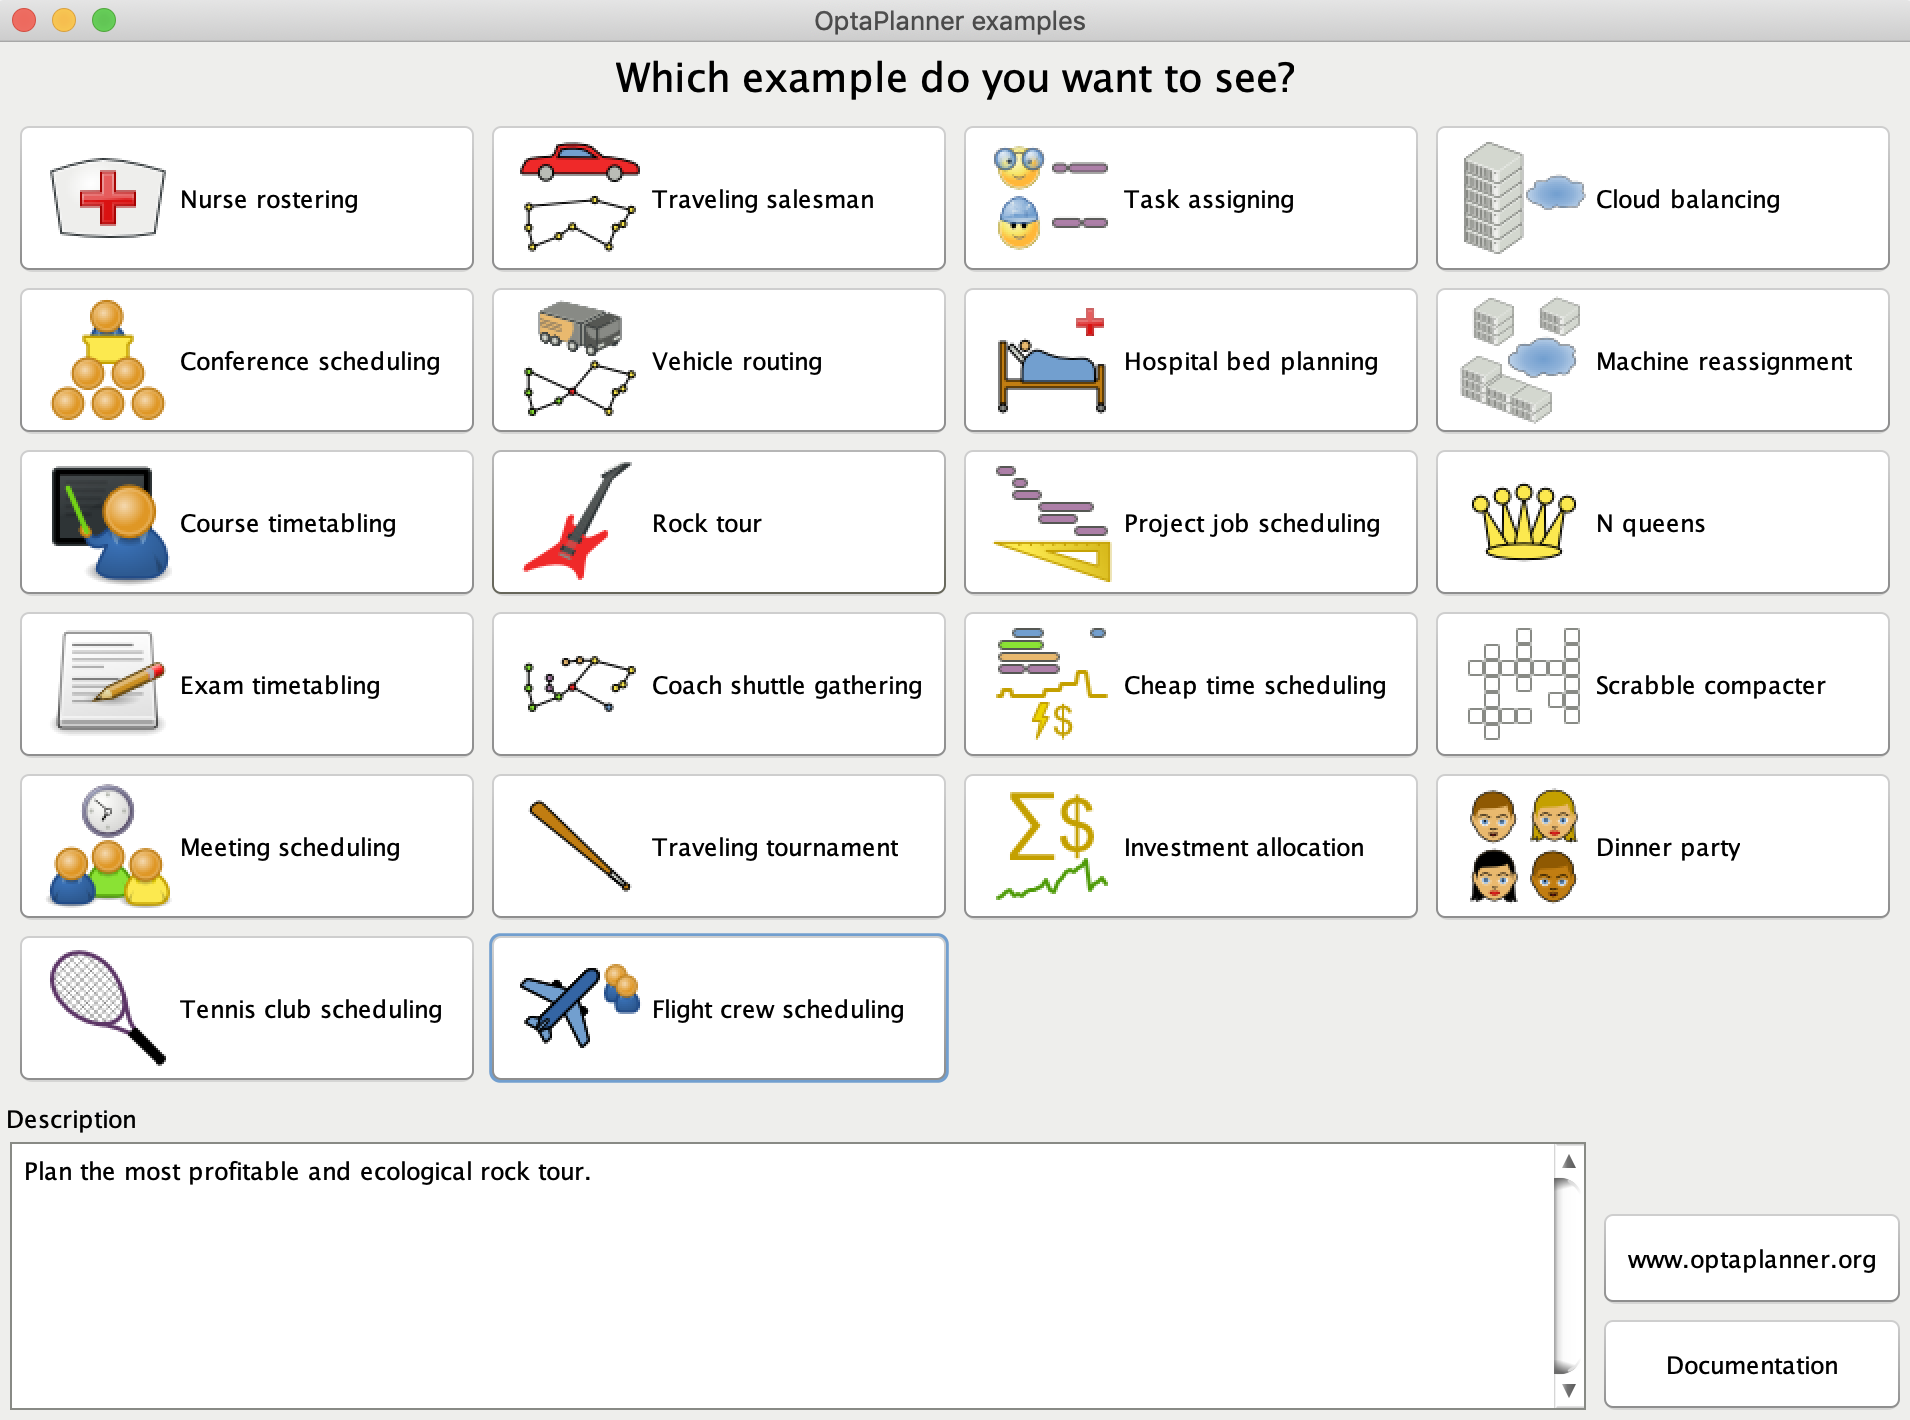
\includegraphics[width=0.6\textwidth]{figures/OPlannerUI.png}
    \caption{OptaPlanner scenarios for the user to choose from. Note that when hoovering over any one of the 22 scenarios, a description of the situation appears. In this case, we have hoovered over ``\textit{Rock tour}''.}
    \label{fig:OP_UI}
\end{figure}
% \begin{figure}
%     \centering
%     \subfloat[\label{fig:task1}]{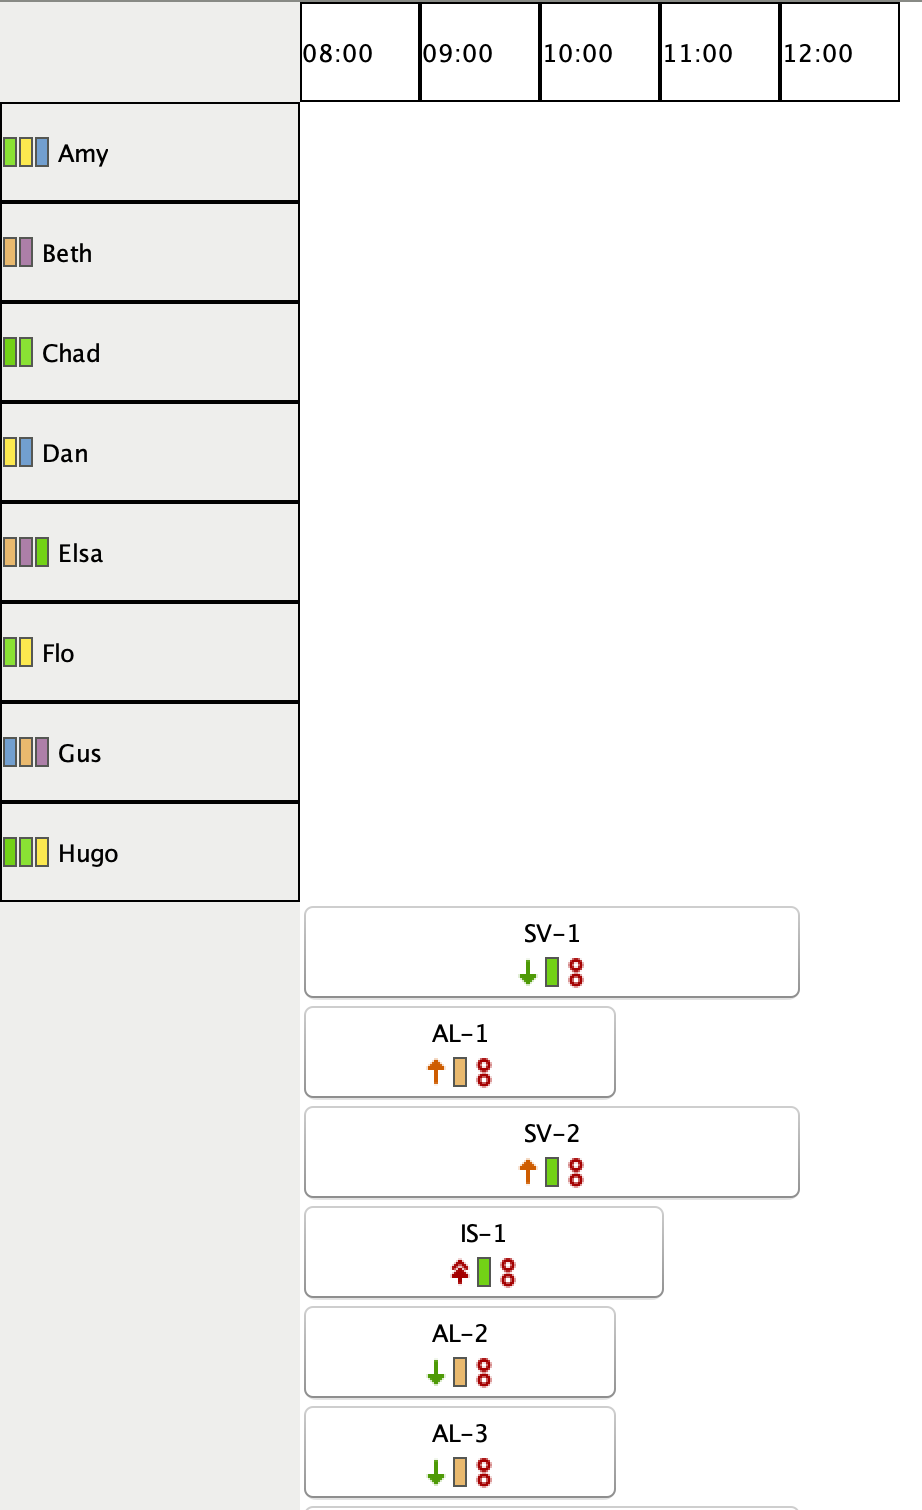
\includegraphics[width=0.48\textwidth]{figures/task-1.png}}
%     \hfill
%     \centering
%     \subfloat[\label{fig:task2}]{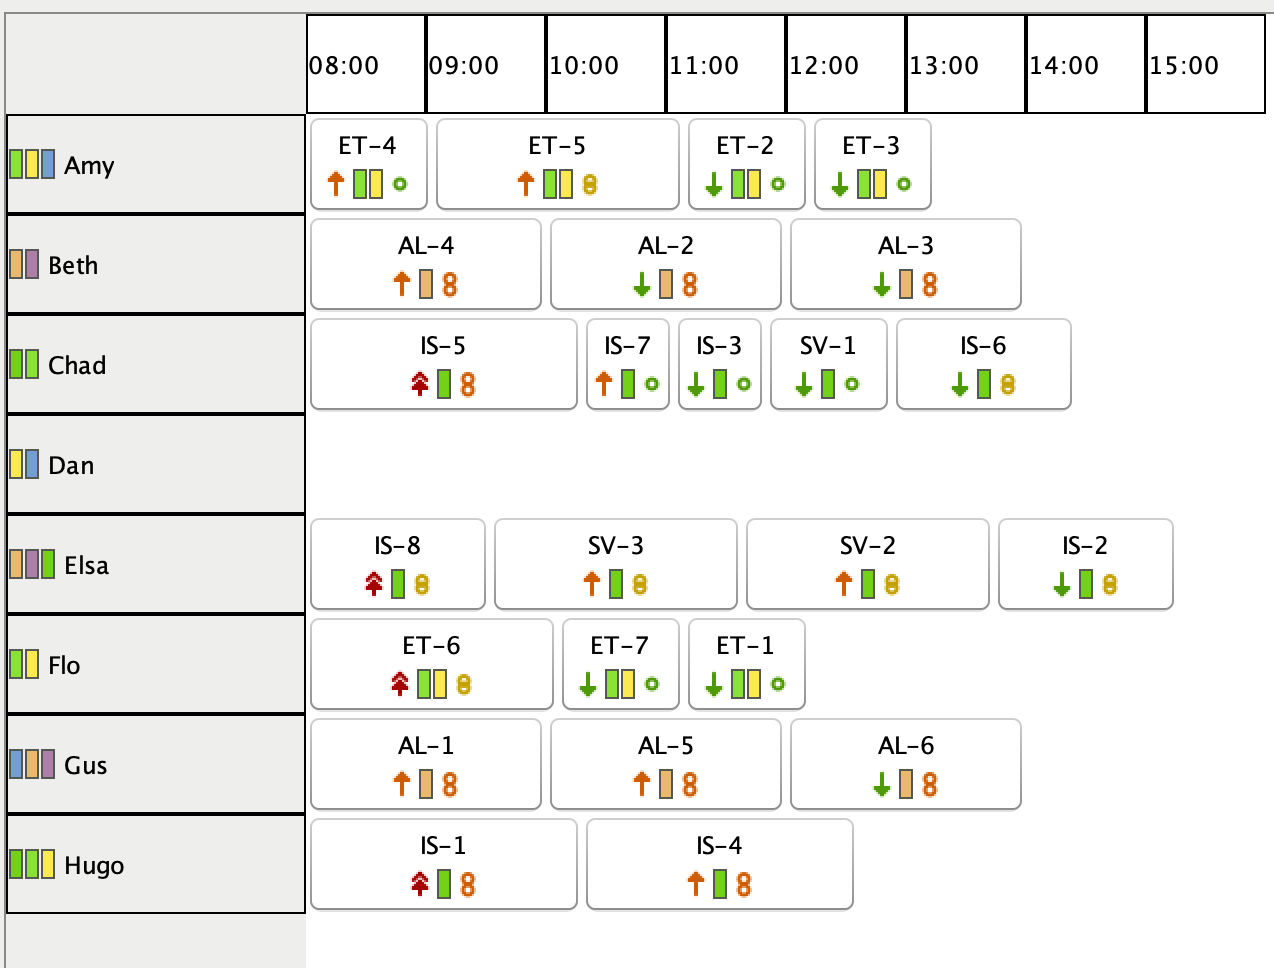
\includegraphics[width=0.48\textwidth]{figures/task-2.png}}
%     \caption{Example application of OptaPlanner to solve a task assigning problem. On the left-handside we see the problem and the conditions that need to be met. On the right-handside we see how OptaPlanner is providing a solution by assigning tasks to each employee.}
%     \label{fig:an_OP_application}
% \end{figure}